\documentclass[12pt,a4paper]{article}

% ── Packages ──────────────────────────────────────────────────
\usepackage[margin=2.5cm]{geometry}
\usepackage{graphicx}
\usepackage{booktabs}
\usepackage{amsmath,amssymb}
\usepackage[ruled,vlined,linesnumbered]{algorithm2e}
\usepackage{tikz}
\usetikzlibrary{positioning,arrows.meta,shapes.multipart,calc}
\usepackage{hyperref}
\usepackage{float}
\usepackage{caption}
\usepackage{enumitem}
\usepackage{multirow}
\usepackage{xcolor}
\usepackage{array}

\hypersetup{
    colorlinks=true,
    linkcolor=blue!70!black,
    citecolor=blue!70!black,
    urlcolor=blue!70!black,
}

% ── Title ─────────────────────────────────────────────────────
\title{
    \textbf{The EVO-ECO Matrix: Simulating Cellular Plasticity\\as a Markov Decision Process}\\[0.5em]
    \large Q-Learning Simulation --- Cancer Cell Survival Strategy\\[1em]
    \normalsize Group A2
}
\author{
    Mohamed Thabet \quad \texttt{100066980}\\
    Nada Morsy \quad \texttt{100049828}\\
    Maryam Albairaq \quad \texttt{100060579}
}
\date{\today}

% ══════════════════════════════════════════════════════════════
\begin{document}
\maketitle
\thispagestyle{empty}
\newpage
\tableofcontents
\newpage

% ──────────────────────────────────────────────────────────────
\section{Abstract}
% ──────────────────────────────────────────────────────────────

This report presents a toy reinforcement-learning simulation that models a single cancer cell as an agent navigating a 32-state Markov Decision Process (MDP). The agent chooses among three actions---\emph{Proliferate}, \emph{Quiesce}, and \emph{Switch} (phenotypic plasticity)---to maximise cumulative survival reward under stochastic therapy, resource, and hazard conditions. Using tabular Q-learning, we sweep the metabolic cost of phenotypic switching ($c_{\text{plast}}$) from 0 to 3 and measure how the learned policy shifts between plasticity-based and proliferation-based survival strategies. Our results show that plasticity (the D$\to$S switch) confers a persistent survival advantage across all tested cost levels, with no sharp tipping-point crossover observed. An episode-count sensitivity analysis at 1{,}000, 10{,}000, and 100{,}000 training episodes confirms that the stochastic environment dynamics dominate the noise in the sweep, and the Switch action functions primarily as a one-time tactical escape from the vulnerable Differentiated phenotype rather than a repeated cycling strategy.

% ──────────────────────────────────────────────────────────────
\section{Introduction}
% ──────────────────────────────────────────────────────────────

Cancer cells exhibit remarkable adaptability during treatment. Two fundamentally different strategies allow tumours to survive therapy:

\begin{enumerate}
    \item \textbf{Phenotypic plasticity} --- reversible, non-genetic switching between a therapy-sensitive differentiated (D) state and a stress-tolerant stem-like (S) state.
    \item \textbf{Genetic mutation} --- irreversible acquisition of drug-resistance alleles during proliferation.
\end{enumerate}

Both strategies carry costs. Plasticity demands metabolic energy for epigenetic reprogramming, while waiting for a random mutation requires continued proliferation under lethal selective pressure. The core research question of this project is:

\begin{quote}
    \emph{At what specific metabolic/fitness cost does reversible phenotypic plasticity become a worse survival strategy than simply proliferating and waiting for a random genetic mutation?}
\end{quote}

We frame the cancer cell as a reinforcement-learning \emph{agent} operating inside an MDP whose states encode the cell's phenotype, genotype, and microenvironment. A tabular Q-learning algorithm learns the optimal survival policy, and a parameter sweep over the plasticity cost reveals the tipping point---if one exists---where the agent abandons the Switch action in favour of Proliferate.

% ──────────────────────────────────────────────────────────────
\section{Experiment Setup}
% ──────────────────────────────────────────────────────────────

\subsection{MDP Formulation}

The simulation is structured as an episodic MDP with the following components:

\begin{itemize}[nosep]
    \item \textbf{State space:} 32 states (5 binary dimensions, $2^5 = 32$).
    \item \textbf{Action space:} 3 discrete actions --- Proliferate, Quiesce, Switch.
    \item \textbf{Transitions:} stochastic, governed by biologically-motivated death probabilities and environment toggles.
    \item \textbf{Reward:} shaped to reflect cellular fitness (survival $+$ reproduction $-$ costs).
    \item \textbf{Termination:} an episode ends when the cell dies or the maximum step count is reached.
\end{itemize}

\subsection{Q-Learning Hyperparameters}

Table~\ref{tab:hyperparams} summarises the Q-learning configuration used throughout the simulation.

\begin{table}[H]
\centering
\caption{Q-learning hyperparameters.}
\label{tab:hyperparams}
\begin{tabular}{lcc}
\toprule
\textbf{Parameter} & \textbf{Symbol} & \textbf{Value} \\
\midrule
Learning rate       & $\alpha$        & 0.1            \\
Discount factor     & $\gamma$        & 0.95           \\
Initial exploration & $\varepsilon_0$ & 1.0            \\
Exploration decay   & ---             & $\times\,0.995$ per episode \\
Minimum exploration & $\varepsilon_{\min}$ & 0.01      \\
\bottomrule
\end{tabular}
\end{table}

\subsection{Training and Evaluation Protocol}

\begin{itemize}[nosep]
    \item \textbf{Training:} 1{,}000 episodes per plasticity-cost level (baseline sweep), each episode up to 1{,}000 steps.
    \item \textbf{Evaluation:} 200 episodes with a fully greedy policy ($\varepsilon = 0$) to measure the learned strategy.
    \item \textbf{Cost sweep:} 30 linearly-spaced values of $c_{\text{plast}} \in [0.0,\; 3.0]$.
    \item \textbf{Starting state:} Differentiated, Sensitive, Therapy ON, Resources High, Hazards High (state index 7) --- the most challenging initial condition.
    \item \textbf{Random seed:} fixed at 42 for reproducibility.
\end{itemize}

% ──────────────────────────────────────────────────────────────
\section{Defined States}
% ──────────────────────────────────────────────────────────────

\subsection{State Space Definition}

Each state in the MDP is a 5-tuple of binary variables:
\[
    \text{State} = (\underbrace{P}_{\text{Phenotype}},\; \underbrace{G}_{\text{Genotype}},\; \underbrace{T}_{\text{Therapy}},\; \underbrace{R}_{\text{Resources}},\; \underbrace{H}_{\text{Hazards}})
\]

Table~\ref{tab:state_dims} lists each dimension with its biological justification.

\begin{table}[H]
\centering
\caption{State dimensions and their biological meaning.}
\label{tab:state_dims}
\begin{tabular}{p{2.3cm}ccp{6.5cm}}
\toprule
\textbf{Dimension} & \textbf{0} & \textbf{1} & \textbf{Biological Justification} \\
\midrule
Phenotype ($P$) & D (Differentiated) & S (Stem-like) & Stemness is a functional state modulated by ecology (e.g.\ hypoxia) rather than a fixed property. D cells are proliferative and therapy-sensitive; S cells are slow-cycling and stress-tolerant. \\
\addlinespace
Genotype ($G$) & Sensitive & Resistant & Therapies select for resistance mutations via classic somatic evolution. Once acquired, resistance is irreversible. \\
\addlinespace
Therapy ($T$) & OFF & ON & Models adaptive therapy scheduling (ON when tumour burden is high, OFF when low). \\
\addlinespace
Resources ($R$) & Low & High & Proxy for oxygen, nutrients, and vasculature (Eco-index resources). \\
\addlinespace
Hazards ($H$) & Low & High & Proxy for therapy intensity and immune predation (Eco-index hazards). \\
\bottomrule
\end{tabular}
\end{table}

\subsection{State Encoding}

States are encoded as a single integer index using the formula:
\[
    \text{index} = P \times 16 + G \times 8 + T \times 4 + R \times 2 + H
\]
This yields indices 0--31. For example, state \texttt{D|G0|Ton|RH|HH} (Differentiated, Sensitive, Therapy ON, Resources High, Hazards High) encodes to $0 \times 16 + 0 \times 8 + 1 \times 4 + 1 \times 2 + 1 = 7$.

\subsection{Death Probability Table}

The probability of cell death at each step depends on the environmental context and phenotype. The biology team defined qualitative levels (low, moderate, high, very high) which were quantified as shown in Table~\ref{tab:death_prob}.

\begin{table}[H]
\centering
\caption{Base death probabilities by condition and phenotype.}
\label{tab:death_prob}
\begin{tabular}{lccc}
\toprule
\textbf{Condition} & \textbf{D cell} & \textbf{S cell} \\
\midrule
Therapy ON + Hazards High + Resources Low   & 0.60 & 0.15 \\
Therapy ON + Hazards High + Resources High  & 0.35 & 0.15 \\
Therapy ON + Hazards Low + Resources Low    & 0.35 & 0.10 \\
Therapy ON + Hazards Low + Resources High   & 0.25 & 0.08 \\
Therapy OFF + Hazards High + Resources Low  & 0.25 & 0.10 \\
Therapy OFF + Hazards High + Resources High & 0.15 & 0.08 \\
Therapy OFF + Hazards Low + Resources Low   & 0.15 & 0.15 \\
Therapy OFF + Hazards Low + Resources High  & 0.05 & 0.05 \\
\bottomrule
\end{tabular}
\end{table}

Two multipliers further modify the base death probability:
\begin{itemize}[nosep]
    \item \textbf{Genetic resistance} ($G=1$): death probability $\times\,0.5$.
    \item \textbf{Quiescence} (action = Quiesce): death probability $\times\,0.5$.
\end{itemize}

\subsection{Environment Dynamics}

The environment dimensions (Therapy, Resources, Hazards) are not controlled by the agent. At each step, each of these three variables independently toggles with probability $p_{\text{toggle}} = 0.10$. This introduces stochasticity into the environment, modelling the unpredictable nature of the tumour microenvironment and treatment schedules.

% ──────────────────────────────────────────────────────────────
\section{Reward Function}
% ──────────────────────────────────────────────────────────────

The reward function is designed to capture cellular fitness as defined by the Merlo/Maley framework: \emph{fitness = survival + reproduction $-$ costs}. The reward at each time step is:

\[
R(s, a) = \begin{cases}
    -10 & \text{if the cell dies (terminal)} \\
    +1 + 2 - c_{\text{plast}} & \text{if Proliferate, survive, and Switch was chosen} \\
    +1 + 2 & \text{if Proliferate and survive} \\
    +1 - 0.1 & \text{if Quiesce and survive} \\
    +1 - c_{\text{plast}} & \text{if Switch and survive}
\end{cases}
\]

More precisely, the reward components are additive:

\begin{table}[H]
\centering
\caption{Reward function components and their biological justification.}
\label{tab:reward}
\begin{tabular}{lcp{7cm}}
\toprule
\textbf{Component} & \textbf{Value} & \textbf{Justification} \\
\midrule
Survival bonus      & $+1$   & Each generation the cell survives contributes to fitness. \\
Proliferation bonus & $+2$   & Successful division increases tumour burden and reproductive fitness. \\
Death penalty       & $-10$  & Terminal penalty reflecting total fitness loss upon death. \\
Plasticity cost     & $-c_{\text{plast}}$ & Metabolic cost of epigenetic reprogramming during phenotype switching. This is the swept parameter. \\
Quiescence cost     & $-0.1$ & Small opportunity cost reflecting foregone growth during dormancy. \\
\bottomrule
\end{tabular}
\end{table}

The \textbf{plasticity cost} $c_{\text{plast}}$ is the central parameter of this study. As $c_{\text{plast}}$ increases, the Switch action becomes increasingly penalised, and the agent is expected to shift its strategy from plasticity-based survival to proliferation-based survival (relying on stochastic genetic mutation for resistance).

% ──────────────────────────────────────────────────────────────
\section{Key Algorithms}
% ──────────────────────────────────────────────────────────────

This section presents the three core algorithms used in the simulation using formal pseudocode notation.

\subsection{Q-Learning with Epsilon-Greedy Policy}

\begin{algorithm}[H]
\caption{Q-Learning Training}\label{alg:qlearning}
\KwIn{Number of episodes $N$, max steps $T$, learning rate $\alpha$, discount $\gamma$, plasticity cost $c_{\text{plast}}$}
\KwOut{Trained Q-table $Q[s, a]$}
Initialise $Q[s, a] \leftarrow 0$ for all $s \in \mathcal{S}$, $a \in \mathcal{A}$\;
$\varepsilon \leftarrow 1.0$\;
\For{episode $= 1$ \KwTo $N$}{
    $s \leftarrow s_0$ \tcp*{Starting state: D|G0|Ton|RH|HH}
    \For{step $= 1$ \KwTo $T$}{
        \tcp{Epsilon-greedy action selection}
        \eIf{$\text{rand}() < \varepsilon$}{
            $a \leftarrow \text{random action from } \mathcal{A}$\;
        }{
            $a \leftarrow \arg\max_{a'} Q[s, a']$\;
        }
        $(s', r, \text{done}) \leftarrow \textsc{Transition}(s, a, c_{\text{plast}})$\;
        \tcp{Bellman update}
        \eIf{\textnormal{done}}{
            $\text{target} \leftarrow r$\;
        }{
            $\text{target} \leftarrow r + \gamma \cdot \max_{a'} Q[s', a']$\;
        }
        $Q[s, a] \leftarrow Q[s, a] + \alpha \cdot (\text{target} - Q[s, a])$\;
        $s \leftarrow s'$\;
        \lIf{\textnormal{done}}{\textbf{break}}
    }
    $\varepsilon \leftarrow \max(\varepsilon_{\min},\; \varepsilon \times 0.995)$\;
}
\Return{$Q$}\;
\end{algorithm}

\subsection{Environment Transition Function}

\begin{algorithm}[H]
\caption{Environment Transition}\label{alg:transition}
\KwIn{State $s$, action $a$, plasticity cost $c_{\text{plast}}$}
\KwOut{Next state $s'$, reward $r$, termination flag \textit{done}}
$(P, G, T, R, H) \leftarrow \textsc{Decode}(s)$\;
$r \leftarrow 0$\;
\tcp{Step 1: Apply action}
\uIf{$a = \textsc{Proliferate}$}{
    \If{$G = 0$ \textbf{and} $\text{rand}() < \mu_0 \times f(\text{Evo})$}{
        $G \leftarrow 1$ \tcp*{Acquire genetic resistance}
    }
}
\uElseIf{$a = \textsc{Quiesce}$}{
    \tcp{No state change; death probability reduced later}
}
\ElseIf{$a = \textsc{Switch}$}{
    $P \leftarrow 1 - P$ \tcp*{Flip phenotype D $\leftrightarrow$ S}
    $r \leftarrow r - c_{\text{plast}}$\;
}
\tcp{Step 2: Stochastic environment toggle}
\lIf{$\text{rand}() < 0.10$}{$T \leftarrow 1 - T$}
\lIf{$\text{rand}() < 0.10$}{$R \leftarrow 1 - R$}
\lIf{$\text{rand}() < 0.10$}{$H \leftarrow 1 - H$}
\tcp{Step 3: Compute death probability}
$p_{\text{death}} \leftarrow \textsc{DeathProb}(T, H, R, P)$\;
\lIf{$G = 1$}{$p_{\text{death}} \leftarrow p_{\text{death}} \times 0.5$}
\lIf{$a = \textsc{Quiesce}$}{$p_{\text{death}} \leftarrow p_{\text{death}} \times 0.5$}
\tcp{Step 4: Survival check}
\If{$\text{rand}() < p_{\text{death}}$}{
    \Return{$(\textsc{Encode}(P,G,T,R,H),\; -10,\; \textbf{true})$}\;
}
\tcp{Step 5: Compute survival reward}
$r \leftarrow r + 1$ \tcp*{Survival bonus}
\lIf{$a = \textsc{Proliferate}$}{$r \leftarrow r + 2$}
\lIf{$a = \textsc{Quiesce}$}{$r \leftarrow r - 0.1$}
\Return{$(\textsc{Encode}(P,G,T,R,H),\; r,\; \textbf{false})$}\;
\end{algorithm}

\subsection{Plasticity Cost Sweep}

\begin{algorithm}[H]
\caption{Plasticity Cost Sweep}\label{alg:sweep}
\KwIn{Cost range $[c_{\min}, c_{\max}]$, number of cost levels $K$, training episodes $N$, evaluation episodes $M$}
\KwOut{Results: average reward, action fractions, survival steps per cost level}
$\text{costs} \leftarrow \textsc{Linspace}(c_{\min}, c_{\max}, K)$\;
\ForEach{$c \in \text{costs}$}{
    $Q \leftarrow \textsc{TrainAgent}(c, N)$ \tcp*{Algorithm~\ref{alg:qlearning}}
    Set $\varepsilon \leftarrow 0$ \tcp*{Greedy evaluation}
    Initialise counters: rewards, action counts, survival steps\;
    \For{eval $= 1$ \KwTo $M$}{
        Run episode with greedy policy using $Q$\;
        Record episode reward, actions taken, steps survived\;
    }
    Store averaged metrics for cost level $c$\;
}
\Return{all results}\;
\end{algorithm}

% ──────────────────────────────────────────────────────────────
\section{Class Diagrams}
% ──────────────────────────────────────────────────────────────

The simulation is implemented in Python using two primary classes: \texttt{BioConfig} (the biology rules engine) and \texttt{QLearningEngine} (the learning agent). Figures~\ref{fig:bioconfig_class} and~\ref{fig:qlearning_class} show their UML class diagrams.

\begin{figure}[H]
\centering
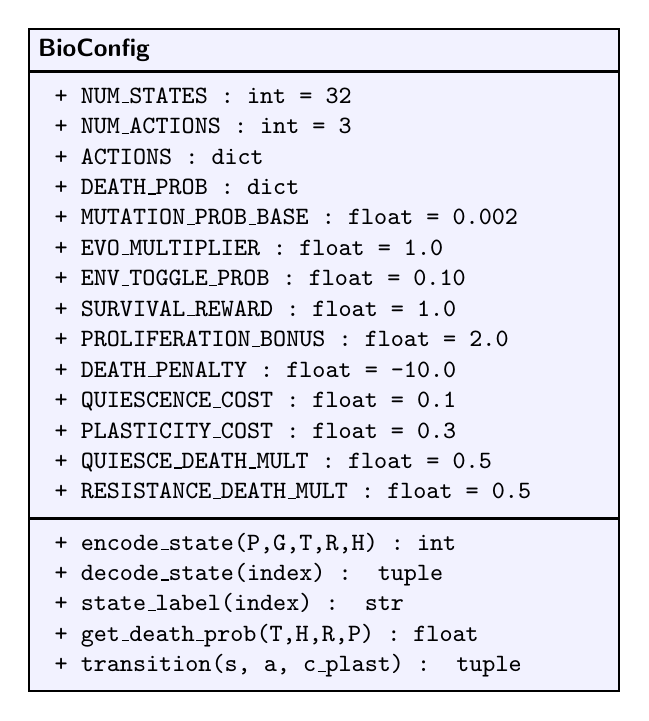
\begin{tikzpicture}[
    class/.style={
        rectangle split,
        rectangle split parts=3,
        rectangle split part align={left,left,left},
        draw,
        thick,
        fill=blue!5,
        minimum width=7.5cm,
        font=\small\ttfamily
    },
    >=Stealth
]
\node[class] (bioconfig) {
    \textbf{\textsf{BioConfig}}
    \nodepart{second}
    \begin{tabular}{l}
    + NUM\_STATES : int = 32 \\
    + NUM\_ACTIONS : int = 3 \\
    + ACTIONS : dict \\
    + DEATH\_PROB : dict \\
    + MUTATION\_PROB\_BASE : float = 0.002 \\
    + EVO\_MULTIPLIER : float = 1.0 \\
    + ENV\_TOGGLE\_PROB : float = 0.10 \\
    + SURVIVAL\_REWARD : float = 1.0 \\
    + PROLIFERATION\_BONUS : float = 2.0 \\
    + DEATH\_PENALTY : float = -10.0 \\
    + QUIESCENCE\_COST : float = 0.1 \\
    + PLASTICITY\_COST : float = 0.3 \\
    + QUIESCE\_DEATH\_MULT : float = 0.5 \\
    + RESISTANCE\_DEATH\_MULT : float = 0.5 \\
    \end{tabular}
    \nodepart{third}
    \begin{tabular}{l}
    + encode\_state(P,G,T,R,H) : int \\
    + decode\_state(index) : tuple \\
    + state\_label(index) : str \\
    + get\_death\_prob(T,H,R,P) : float \\
    + transition(s, a, c\_plast) : tuple \\
    \end{tabular}
};
\end{tikzpicture}
\caption{UML class diagram for \texttt{BioConfig} --- the biology rules engine.}
\label{fig:bioconfig_class}
\end{figure}

\begin{figure}[H]
\centering
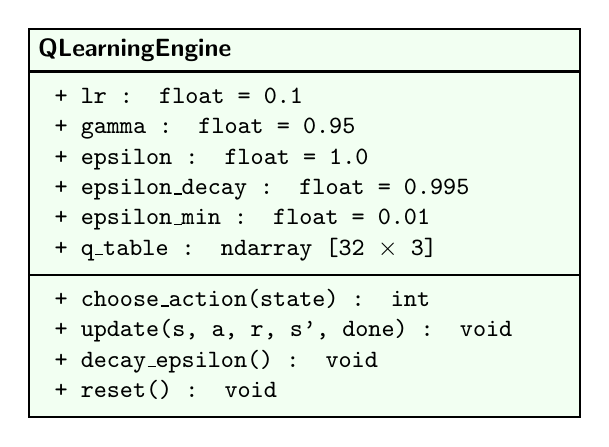
\begin{tikzpicture}[
    class/.style={
        rectangle split,
        rectangle split parts=3,
        rectangle split part align={left,left,left},
        draw,
        thick,
        fill=green!5,
        minimum width=7cm,
        font=\small\ttfamily
    },
    >=Stealth
]
\node[class] (qlearning) {
    \textbf{\textsf{QLearningEngine}}
    \nodepart{second}
    \begin{tabular}{l}
    + lr : float = 0.1 \\
    + gamma : float = 0.95 \\
    + epsilon : float = 1.0 \\
    + epsilon\_decay : float = 0.995 \\
    + epsilon\_min : float = 0.01 \\
    + q\_table : ndarray [32 $\times$ 3] \\
    \end{tabular}
    \nodepart{third}
    \begin{tabular}{l}
    + choose\_action(state) : int \\
    + update(s, a, r, s', done) : void \\
    + decay\_epsilon() : void \\
    + reset() : void \\
    \end{tabular}
};
\end{tikzpicture}
\caption{UML class diagram for \texttt{QLearningEngine} --- the Q-learning agent.}
\label{fig:qlearning_class}
\end{figure}

\texttt{BioConfig} acts as a static configuration and physics engine: it encodes/decodes states, stores all biology-defined parameters (death probabilities, reward values, mutation rates), and implements the \texttt{transition()} function that governs how the environment responds to agent actions. \texttt{QLearningEngine} is the learning agent that maintains a $32 \times 3$ Q-table and implements the epsilon-greedy policy with Bellman updates.

% ──────────────────────────────────────────────────────────────
\section{Simulation Flow Diagram}
% ──────────────────────────────────────────────────────────────

Figure~\ref{fig:flowchart} shows the complete decision and evolution model flowchart, illustrating how a single time step is processed in the simulation.

\begin{figure}[H]
\centering
\includegraphics[width=\textwidth]{Full_Flow_Chart.png}
\caption{Cancer Cell Decision and Evolution Model --- full simulation flow diagram. At each step, the environment state is evaluated, the agent selects an action via its Q-table policy, the action is applied (with possible mutation during proliferation or phenotype flip during switching), the environment stochastically toggles, a death check is performed, and the reward is computed.}
\label{fig:flowchart}
\end{figure}

The flow proceeds as follows:
\begin{enumerate}[nosep]
    \item \textbf{Evaluate environment} --- read the current 5-dimensional state $(P, G, T, R, H)$.
    \item \textbf{Check if alive} --- if the cell died in the previous step, the episode ends with reward $-10$.
    \item \textbf{Choose action} --- the agent's policy (epsilon-greedy over the Q-table) selects Proliferate, Quiesce, or Switch.
    \item \textbf{Apply action} --- Proliferate may trigger a mutation ($G: 0 \to 1$); Switch flips the phenotype ($P: D \leftrightarrow S$) at a metabolic cost; Quiesce reduces hazard exposure.
    \item \textbf{Environment toggle} --- Therapy, Resources, and Hazards each independently flip with 10\% probability.
    \item \textbf{Death check} --- a survival roll is made against the death probability (modified by genotype and quiescence).
    \item \textbf{Compute reward} --- survival, proliferation, plasticity, and quiescence components are summed.
    \item \textbf{Advance} --- move to the next time step with the updated state.
\end{enumerate}

% ──────────────────────────────────────────────────────────────
\section{Interactive Step-Through Viewer}
% ──────────────────────────────────────────────────────────────

To facilitate pedagogical inspection of the Q-learning process, the simulation includes an interactive step-through viewer built with Tkinter (Figure~\ref{fig:viewer}).

\begin{figure}[H]
\centering
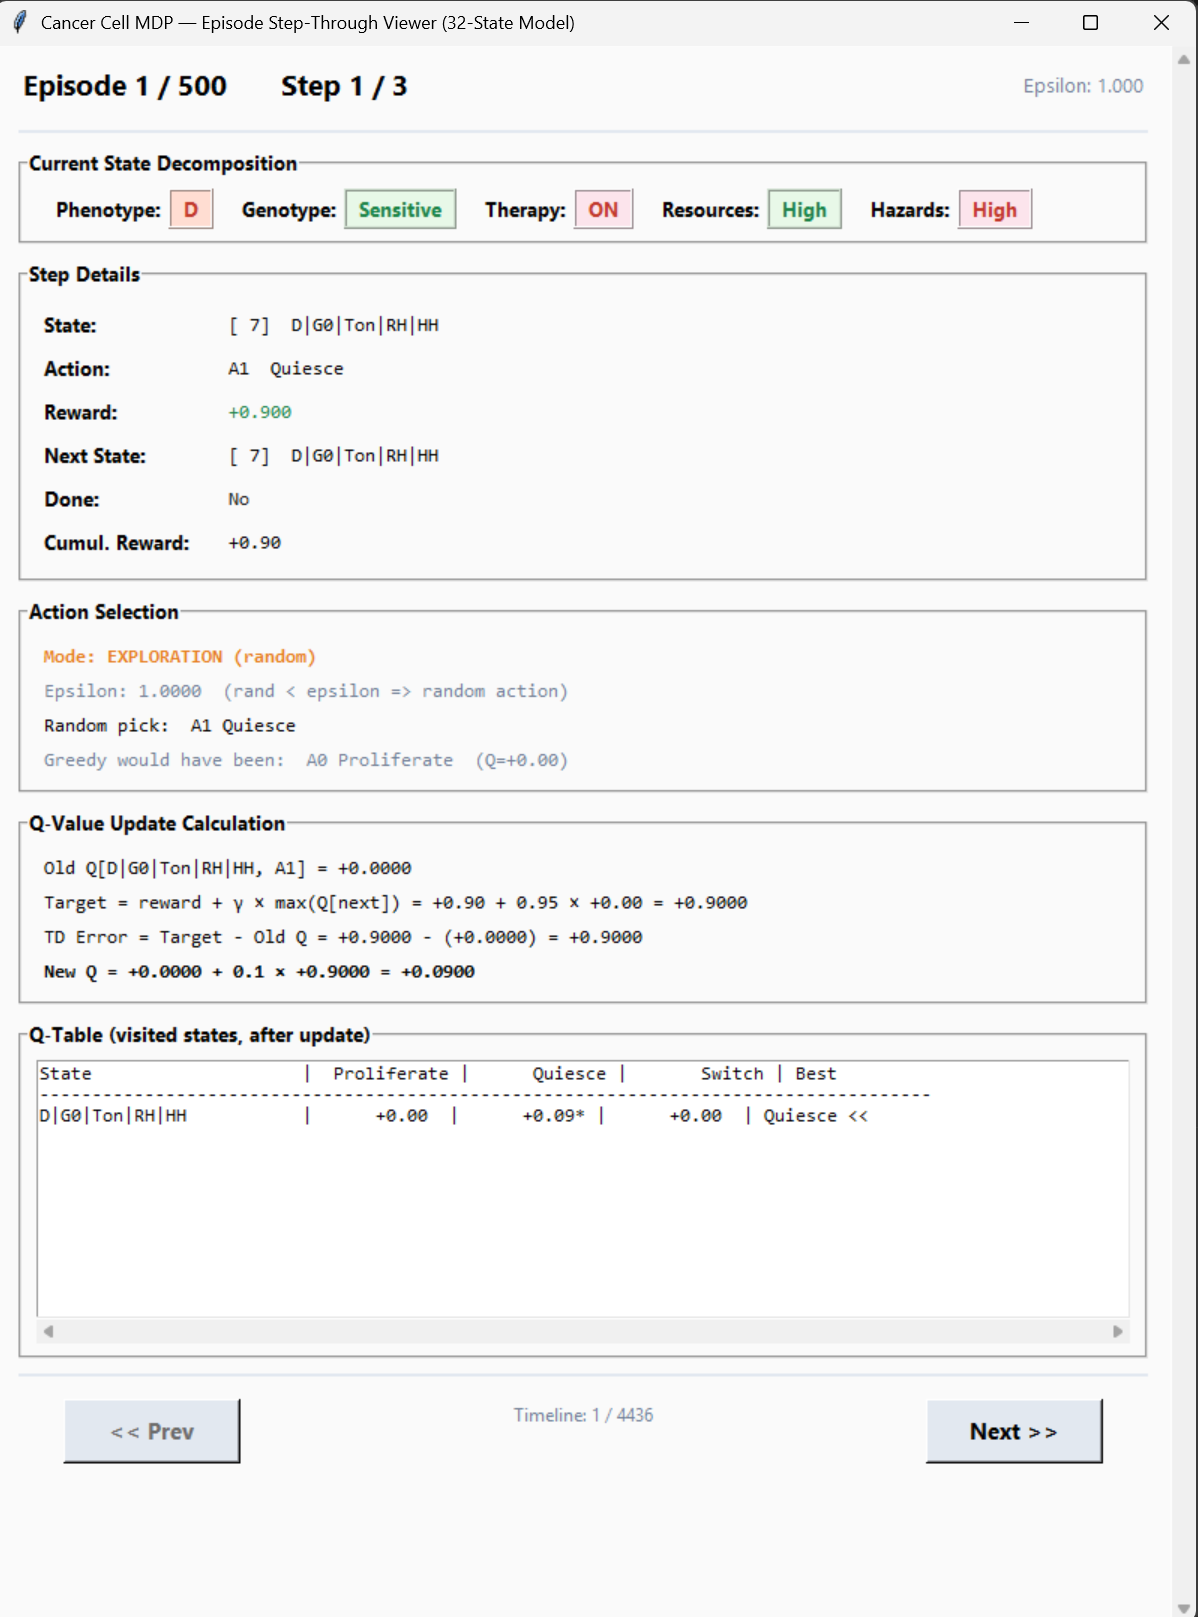
\includegraphics[width=0.55\textwidth]{toy-screenshot.png}
\caption{Screenshot of the Interactive Step-Through Viewer.}
\label{fig:viewer}
\end{figure}

The viewer records 500 episodes of training and allows the user to navigate through every individual step using \textbf{Previous}/\textbf{Next} buttons (or arrow keys). At each step, the viewer displays:

\begin{itemize}[nosep]
    \item \textbf{Current State Decomposition} --- colour-coded badges showing the value of each state dimension (Phenotype, Genotype, Therapy, Resources, Hazards).
    \item \textbf{Step Details} --- the current state index, chosen action, immediate reward, next state, termination flag, and cumulative episode reward.
    \item \textbf{Action Selection} --- whether the action was chosen via \emph{exploration} (random, shown in orange) or \emph{exploitation} (greedy, shown in green), along with the current epsilon value and what the greedy choice would have been.
    \item \textbf{Q-Value Update Calculation} --- the full Bellman update arithmetic: old Q-value, target computation ($r + \gamma \max Q'$), TD error, and the resulting new Q-value.
    \item \textbf{Q-Table} --- the current Q-table showing all visited states, with the active state highlighted and the greedy-best action marked.
\end{itemize}

Between episodes, a \textbf{summary screen} reports the total steps survived, cumulative reward, final state, and the episode outcome (Cell Died, Genetically Resistant, or Survived to max steps).

% ──────────────────────────────────────────────────────────────
\section{Simulation Outcomes and Results}
% ──────────────────────────────────────────────────────────────

\subsection{Tipping-Point Sweep}

Figure~\ref{fig:tipping} shows the results of the plasticity cost sweep across 30 cost levels in $[0.0, 3.0]$.

\begin{figure}[H]
\centering
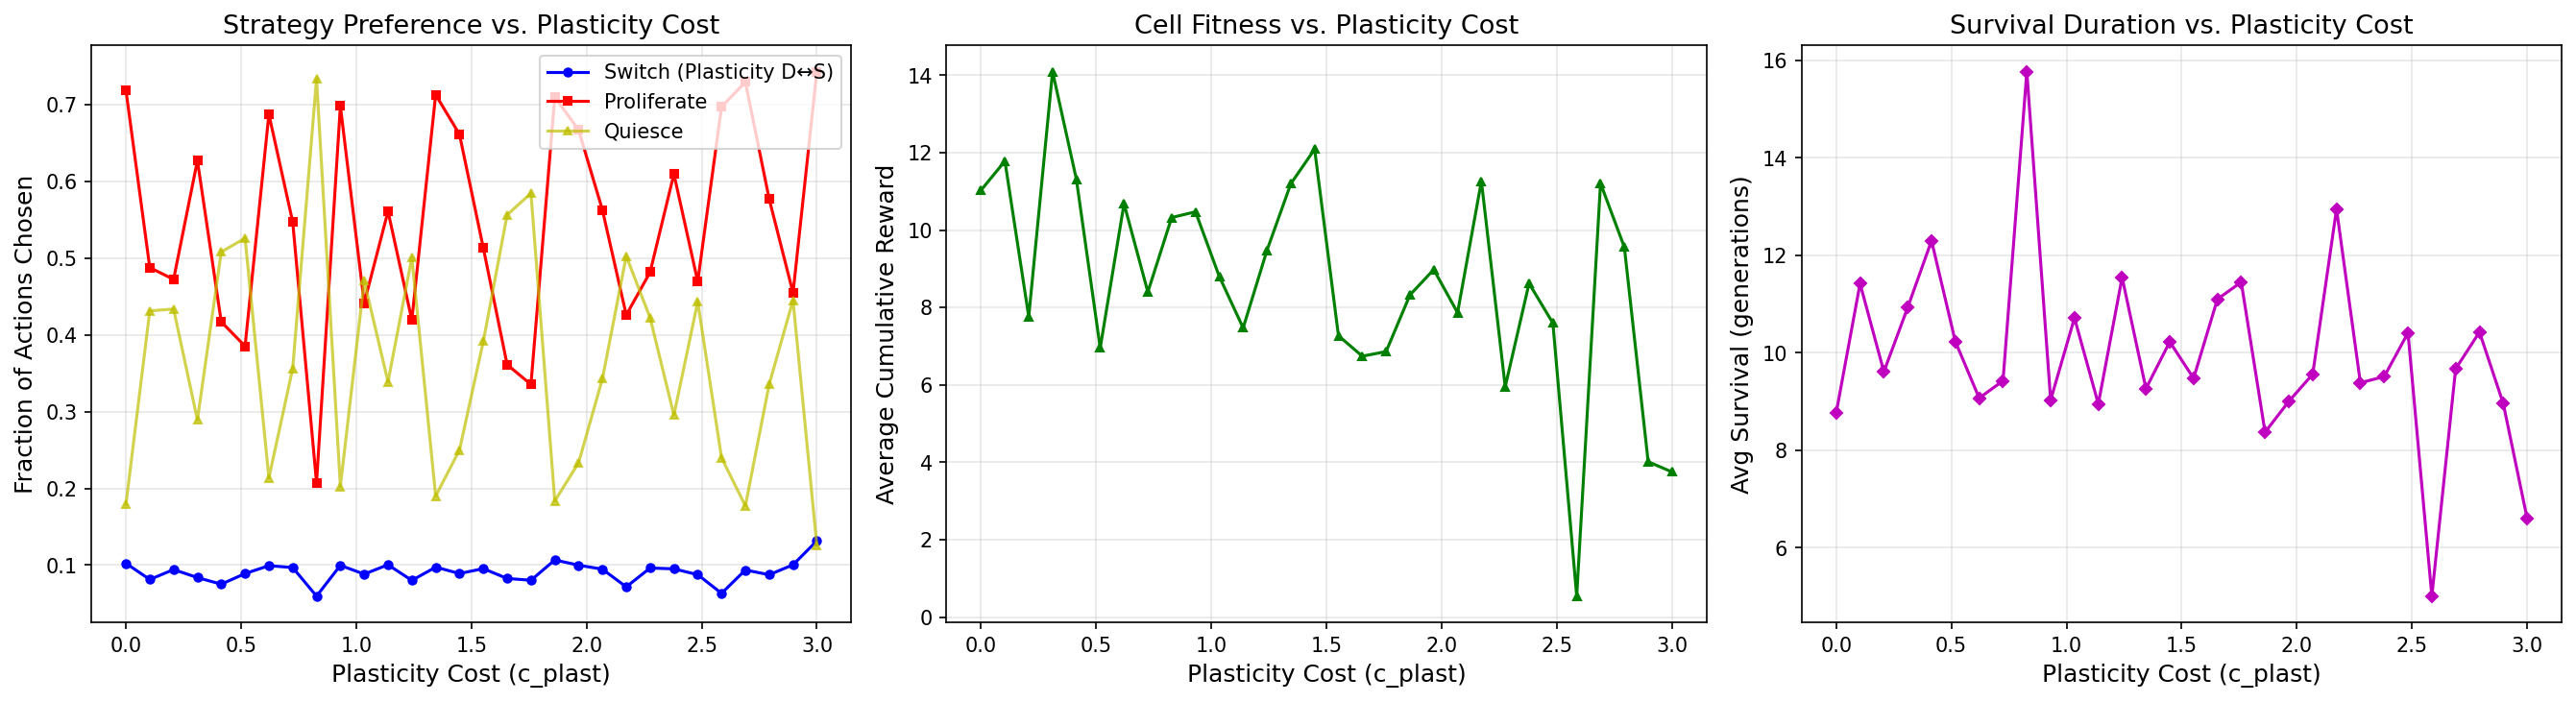
\includegraphics[width=\textwidth]{tipping_point.png}
\caption{Tipping-point sweep results. \textbf{Left:} Strategy preference (fraction of actions chosen) vs.\ plasticity cost. \textbf{Centre:} Average cumulative reward (cell fitness). \textbf{Right:} Average survival duration in steps.}
\label{fig:tipping}
\end{figure}

\subsubsection{Strategy Preference (Left Panel)}

The \textbf{Proliferate} action (red) dominates across all cost levels, accounting for 35--75\% of actions. \textbf{Quiesce} (yellow) serves as a secondary survival strategy, fluctuating between 12--73\%. The \textbf{Switch} action (blue) maintains a consistent fraction of approximately 8--13\% regardless of plasticity cost.

Crucially, \emph{no sharp crossover} between Switch and Proliferate is observed. The Switch fraction does not decline monotonically as $c_{\text{plast}}$ increases. This indicates that plasticity is used as a tactical, one-time escape from the Differentiated phenotype rather than a repeated cycling strategy.

\subsubsection{Cell Fitness (Centre Panel)}

Average cumulative reward fluctuates between 0.5 and 14.1 across cost levels, with no clear downward trend as $c_{\text{plast}}$ increases. The high variance reflects the stochastic nature of the environment (10\% toggle probability per dimension per step) and the short average episode length (8--16 steps).

\subsubsection{Survival Duration (Right Panel)}

Average survival ranges from 5 to 16 steps, again with high variance and no systematic trend with plasticity cost. This confirms that the environment's stochasticity dominates the agent's survival prospects.

\subsection{Q-Table Analysis}

Table~\ref{tab:qtable_comparison} compares the learned policy at low ($c_{\text{plast}} = 0.1$) and high ($c_{\text{plast}} = 2.0$) plasticity costs for the D-phenotype states (the states where the Switch decision is most consequential).

\begin{table}[H]
\centering
\caption{Learned best action for D-phenotype states at low vs.\ high plasticity cost.}
\label{tab:qtable_comparison}
\begin{tabular}{lcc}
\toprule
\textbf{State} & \textbf{Best Action ($c=0.1$)} & \textbf{Best Action ($c=2.0$)} \\
\midrule
D|G0|Toff|RL|HL & Proliferate & Quiesce \\
D|G0|Toff|RL|HH & Proliferate & Switch \\
D|G0|Toff|RH|HL & Switch & Switch \\
D|G0|Toff|RH|HH & Switch & Switch \\
D|G0|Ton|RL|HL  & Switch & Switch \\
D|G0|Ton|RL|HH  & Switch & Switch \\
D|G0|Ton|RH|HL  & Switch & Switch \\
D|G0|Ton|RH|HH  & Switch & Switch \\
\bottomrule
\end{tabular}
\end{table}

Even at $c_{\text{plast}} = 2.0$, the agent still prefers Switch in 7 out of 8 D-phenotype states. This is because the survival advantage of transitioning from D (high death probability) to S (low death probability) is so large that it outweighs even a substantial metabolic cost. For example, under Therapy ON + Hazards High + Resources Low, D cells face a 60\% death probability while S cells face only 15\% --- a fourfold reduction that easily justifies a one-time cost of 2.0 given the $-10$ death penalty.

Once in the S phenotype, the agent predominantly chooses \textbf{Proliferate} (gaining the $+3$ reward per step) and rarely switches back to D.

\subsection{Episode Count Sensitivity Analysis}

To investigate whether the noisy sweep results reflect insufficient training, we repeated the full sweep at three training durations: 1{,}000, 10{,}000, and 100{,}000 episodes per cost level.

\begin{figure}[H]
\centering
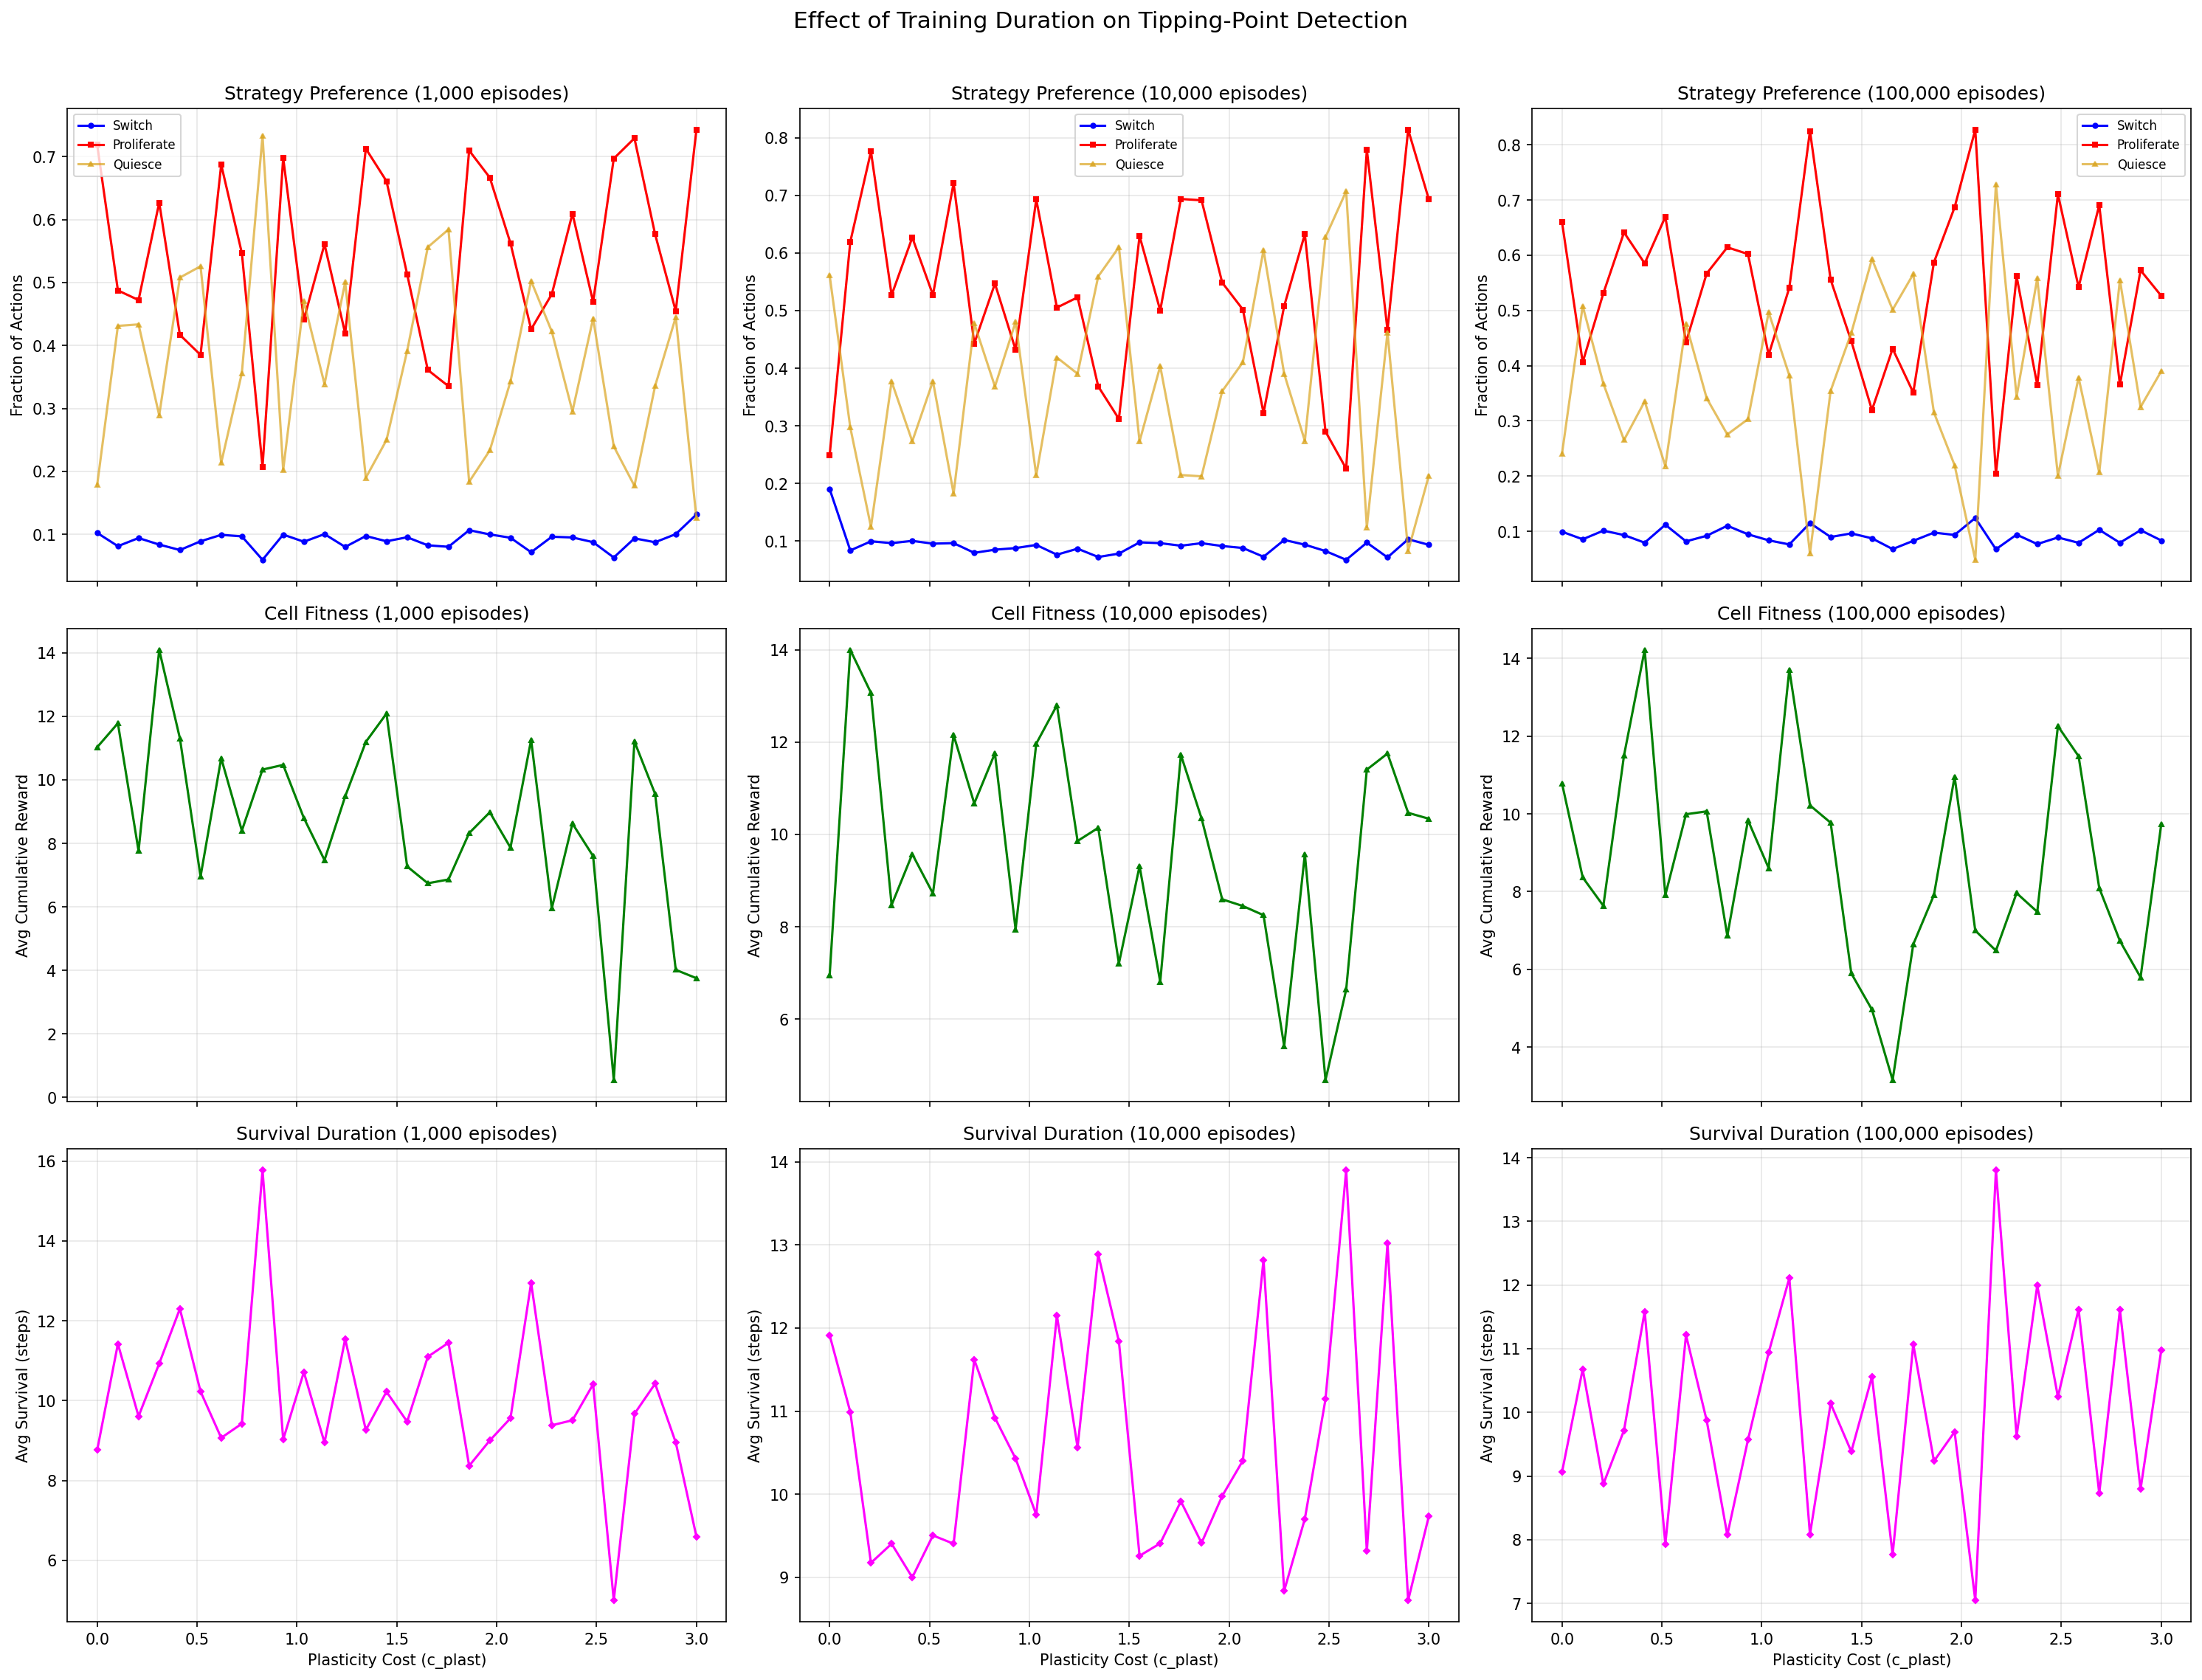
\includegraphics[width=\textwidth]{tipping_point_episodes.png}
\caption{Effect of training duration on tipping-point detection. Columns: 1{,}000 / 10{,}000 / 100{,}000 episodes. Rows: strategy preference, cell fitness, survival duration.}
\label{fig:episodes}
\end{figure}

Key observations from Figure~\ref{fig:episodes}:
\begin{enumerate}[nosep]
    \item \textbf{Strategy preference remains noisy} across all training durations. Even at 100{,}000 episodes, the Proliferate and Quiesce fractions fluctuate substantially, while Switch remains consistently low (8--13\%).
    \item \textbf{No tipping point emerges} at any training duration. The absence of a Switch-vs-Proliferate crossover is a robust finding, not an artefact of under-training.
    \item \textbf{Cell fitness and survival} show similar variance across all three durations, confirming that the stochastic environment dynamics (not learning convergence) drive the noise.
\end{enumerate}

The persistence of noise is expected: with 10\% toggle probability on three binary dimensions, the environment effectively randomises every $\sim$10 steps, creating a non-stationary backdrop that limits the agent's ability to learn long-horizon strategies. The Q-table converges for the \emph{immediate} tactical decision (Switch when D, Proliferate when S) but cannot predict far-future environment states.

% ──────────────────────────────────────────────────────────────
\section{Discussion}
% ──────────────────────────────────────────────────────────────

\subsection{Key Findings}

\begin{enumerate}
    \item \textbf{Plasticity provides a persistent survival advantage.} The D$\to$S switch is so beneficial (reducing death probability by 2--4$\times$) that the agent prefers it even at plasticity costs as high as $c_{\text{plast}} = 3.0$. This suggests that in environments with strong differential selection between phenotypes, phenotypic plasticity is a robustly optimal strategy.

    \item \textbf{No sharp tipping point exists in this model.} Unlike the expected crossover where Switch usage drops to zero as cost increases, the Switch action persists as a minority but consistent strategy. The ``tipping point'' is better characterised as a gradual shift: at higher costs, the agent uses Switch \emph{only} in the most dangerous D-states (Therapy ON, Hazards High) rather than in all D-states.

    \item \textbf{The agent learns a two-phase strategy:} (1) Immediately switch from D to S if starting in a D-state, then (2) Proliferate aggressively in the S phenotype to accumulate fitness. This is a rational policy given that S cells have dramatically lower death probabilities.

    \item \textbf{Genetic mutation plays a negligible role} at the base mutation rate of $\mu_0 = 0.002$. Across 1{,}000 episodes of $\sim$10 steps each, the expected number of mutation events is approximately $1{,}000 \times 10 \times 0.002 \approx 20$, which is too few for the Q-table to learn reliable resistance-dependent strategies.
\end{enumerate}

\subsection{Biological Interpretation}

The simulation results align with biological observations that cancer stem-like cells are inherently more resistant to therapy. The model confirms that:
\begin{itemize}[nosep]
    \item When the fitness differential between phenotypes is large, plasticity is always advantageous regardless of metabolic cost.
    \item A tipping point would require either (a) a smaller D-vs-S survival differential, (b) a higher mutation rate making genetic resistance more accessible, or (c) longer episodes where the cumulative cost of repeated switching becomes significant.
\end{itemize}

\subsection{Limitations}

\begin{itemize}[nosep]
    \item \textbf{Single-cell model:} No cell-cell interactions, spatial structure, or population dynamics.
    \item \textbf{Binary state dimensions:} Real biological variables are continuous.
    \item \textbf{Environment stochasticity:} The 10\% toggle probability was an assumption, not derived from data.
    \item \textbf{Short episodes:} Average survival of $\sim$10 steps limits the horizon over which plasticity costs accumulate.
    \item \textbf{Tabular Q-learning:} With only 32 states, the model is tractable but may miss complex state interactions that a function-approximation approach could capture.
\end{itemize}

% ──────────────────────────────────────────────────────────────
\section{AI Tools Used}
% ──────────────────────────────────────────────────────────────

The following artificial intelligence tools were used in the development of this project:

\begin{itemize}
    \item \textbf{Claude} (Anthropic) --- Used for computational development including Python code implementation, debugging, simulation architecture design, interactive viewer development, and report generation.
    \item \textbf{ChatGPT} (OpenAI) --- Used for biological model specification, literature-informed rule design, reward function formulation, and research assistance in defining biologically accurate state transitions and death probabilities.
\end{itemize}

Both tools were used as assistive aids under human supervision. All biological rules were validated by the biology team members, and all code was reviewed and tested by the computational team members.

% ──────────────────────────────────────────────────────────────
\section{References}
% ──────────────────────────────────────────────────────────────

\begin{enumerate}[label={[\arabic*]}]
    \item \textbf{GitHub Repository:} \url{https://github.com/mohamedG09/rl-cancer} --- Full source code, Jupyter notebook, and generated figures.
    \item Merlo, L.M.F., Pepper, J.W., Reid, B.J., Maley, C.C. (2006). Cancer as an evolutionary and ecological process. \textit{Nature Reviews Cancer}, 6(12), 924--935.
    \item Watkins, C.J.C.H., Dayan, P. (1992). Q-learning. \textit{Machine Learning}, 8(3), 279--292.
    \item Sutton, R.S., Barto, A.G. (2018). \textit{Reinforcement Learning: An Introduction}. 2nd ed. MIT Press.
\end{enumerate}

\end{document}
